\documentclass[a4paper,12pt,oneside]{article}

\usepackage[left=1.0in, right=1.0in, top=1.0in, bottom=1.0in]{geometry}

\usepackage[toc,page]{appendix}
\usepackage{amsmath}
\usepackage{amsfonts}
\usepackage{amssymb}
\usepackage{amsthm}
\usepackage{color}
\usepackage{graphics}
\usepackage{graphicx}
\usepackage{epsfig}
\usepackage{epstopdf}
\epstopdfsetup{update}
\usepackage{float}
\usepackage{rotating}
\usepackage{array}
\usepackage{textcomp}
\usepackage{bbm}
\usepackage{fancyref}
\usepackage{xcolor}
\usepackage{rotating}
\usepackage[noadjust]{cite} % basic fos bibliography [1]-[5]
\usepackage{bm}
\usepackage{mathtools}
\usepackage{multirow}
\usepackage{array}
\usepackage{longtable}
\usepackage{hhline}
\usepackage{indentfirst}
\usepackage{framed}
\usepackage[hidelinks]{hyperref}
\usepackage{tcolorbox}
\usepackage{pgfplots}
\usepackage{tikz}
\usetikzlibrary{calc,positioning,shapes,shadows,arrows,fit}

\widowpenalty=1000
\clubpenalty=1000

\usepackage{environ}
\NewEnviron{gg_box}{%
  \begin{tcolorbox}[colback=black!10, colframe=white!80!]
    \BODY
  \end{tcolorbox}
}

\NewEnviron{bw_box}{%
  \begin{tcolorbox}[colback=white!10, colframe=black!80!, arc=0pt,outer arc=0pt]
    \BODY
  \end{tcolorbox}
}

\NewEnviron{gw_box}{%
  \begin{tcolorbox}[colback=white!10, colframe=black!10!]
    \BODY
  \end{tcolorbox}
}

\NewEnviron{bg_box}{%
  \begin{tcolorbox}[colback=black!10, colframe=black!80!, arc=0pt,outer arc=0pt]
    \BODY
  \end{tcolorbox}
}



%\usepackage{fontspec}
%\setmainfont{cmr12}


%\usepackage{algorithm}
%\usepackage{algpseudocode}
%\usepackage{algcompatible}
%\usepackage{pifont}
%\usepackage[]{algorithm2e}
%\usepackage{stmaryrd}
%\usepackage{subcaption}


\theoremstyle{definition}
\newtheorem{definition}{Definition}[section] %definition
\newtheorem{remark}{Remark}[section] % remark
\newtheorem{theorem}{Theorem}[section] % theorem
\newtheorem{example}{Example}[section] % example
\newtheorem{assumption}{Assumption}[section] % example
\newtheorem{problem}{Problem}[section]
\newtheorem{lemma}{Lemma}[section]

%\newtheorem{theorem}{Theorem}[section] % theorem


\newcolumntype{C}[1]{>{\centering\let\newline\\\arraybackslash}m{#1}}

\makeatletter
\def\BState{\State\hskip-\ALG@thistlm}
\makeatother

\newcommand{\note}[1]{{\color{red}  #1}}
\newcommand{\mat}[1]{\bm{\mathit{#1}}}
\newcommand{\vect}[1]{\bm{\mathbf{#1}}}

%\hypersetup{colorlinks=false, linkbordercolor={0 0 1}}












\title{\textbf{Multi-Robot Control by
Utilizing Distributed Model Predictive Controllers}}
%
\author{KTH Royal Institute of Technology \\
  School of Electrical Engineering \\
  Department of Automatic Control \\ \\
Student: Alexandros Filotheou (\href{mailto: alefil@kth.se}{alefil@kth.se}) \\
Supervisor: Alexandros Nikou (\href{mailto: anikou@kth.se}{anikou@kth.se}) \\
Examiner: Dimos Dimarogonas (\href{mailto: dimos@kth.se}{dimos@kth.se}) \\}

\date{\today}

\begin{document}

\maketitle

\begin{abstract}
	This paper addresses the problem of position- and orientation-based formation
  control of a class of second-order nonlinear multi-agent systems in $3$D
  space, under static and undirected communication topologies. More
  specifically, we design a decentralized control protocol for each agent in
  the sense that each agent uses only local information from its neighbors to
  calculate its own control signal. Additionally, by introducing certain
  inter-agent distance constraints, we guarantee collision avoidance both
  between among the agents and between the agents and possible obstacles of the
  workspace. Connectivity maintenance between agents that are initially
  connected is also achieved by the proposed controller scheme. Finally,
  simulation results verify the  performance of the proposed controllers.
\end{abstract}

\newpage
\tableofcontents
\newpage


\section{Introduction}

  \noindent formation of multi-agent systems, mpc intro etc. \\

\noindent motivation why we need mpc controllers...  \\

\noindent In many control problems it is desired to design a stabilizing
feedback such that a performance criterion is minimized while satisfying
constraints on the controls and the states. Ideally one would look for a
closed solution for the feedback law satisfying the constraints while
optimizing the performance. However, typically the optimal feedback law
cannot be found analytically, even in the unconstrained case, since it involves
the solution of the corresponding Hamilton-Jacobi-Bellman partial differential
equations. One approach to circumvent this problem is the repeated solution of
an open-loop optimal control problem for a given state. The first part of the
resulting open-loop input signal is implemented and the whole process is
repeated. Control approaches using this strategy are referred to as Model
Predictive Control (MPC).

  \newpage

%-------------------------------------------------------------------------------
\part{The problem}
\newpage

  \section{Notation and Preliminaries}
    \label{sec:notation_reliminaries}

    \subsection{Notation}

The set of positive integers is denoted by $\mathbb{N}$. The real $n$-coordinate
space, with $n\in\mathbb{N}$, is denoted by $\mathbb{R}^n$;
$\mathbb{R}^n_{\geq 0}$ and $\mathbb{R}^n_{> 0}$ are the sets of real
$n$-vectors with all elements nonnegative and positive, respectively. Given a
set $S$, we denote as $\lvert S\lvert$ its cardinality. The notation
$\|\vect{x}\|$ is used for the Euclidean norm of a vector
$\vect{x} \in \mathbb{R}^n$. Given a symmetric matrix
$\mat{A} = \mat{A}^T, \lambda_{\text{min}}(\mat{A})$
denotes the minimum eigenvalue of $\mat{A}$, respectively, where
$\sigma(\mat{A})$ is the set of all the eigenvalues of
$\mat{A}$ and $\text{rank}(\mat{A})$ is its rank. Given two sets $S_1$ and $S_2$,
the operation $S_1 \oplus S_2$ denotes the Minkowski addition, defined by
$S_1 \oplus S_2 = \{s_1 + s_2 : s_1 \in S_1, s_2 \in S_2$. Define by
$\vect{1}_n \in \mathbb{R}^n, \mat{I_n} \in \mathbb{R}^{n \times n},
\mat{0}_{m \times n} \in \mathbb{R}^{m \times n}$
the column vector with all entries $1$, the unit matrix and the $m \times n$
matrix with all entries zeros, respectively.
A matrix $\mat{A} \in \mathbb{R}^{n \times n}$ is called skew-symmetric if and only
if $\mat{A}^\top = -\mat{A}$.
$\mathcal{B}(\vect{c},r) \overset{\Delta}{=} \{\vect{x} \in \mathbb{R}^3: \|\vect{x}-\vect{c}\| \leq r\}$
is the $3$D sphere of radius $r \in \mathbb{R}_{\ge 0}$ and center
$\vect{c}\in\mathbb{R}^{3}$.

The vector expressing the coordinates of the origin of frame $\{j\}$ in
frame $\{i\}$ is denoted by $\vect{p}_{j \triangleright i}$. When this vector is
expressed in 3D space in a third frame, frame $\{k\}$, it is denoted by
$\vect{p}_{j \triangleright i}^{k}$.
%Given $\vect{a}\in\mathbb{R}^3$, $\mat{S}(\vect{a})$ is the skew-symmetric
%matrix defined according to $\mat{S}(\vect{a})\vect{b} = \vect{a}\times \vect{b}$.
The angular velocity of frame $\{j\}$ with respect to frame $\{i\}$, expressed
in frame $\{k\}$ coordinates, is denoted by
$\vect{\omega}^k_{j \triangleright i}\in \mathbb{R}^{3}$.
We also use the notation $\mathbb{M} = \mathbb{R}^3\times \mathbb{T}^3$.
We further denote as $\vect{q}_{j \triangleright i} \in \mathbb{T}^3$
the Euler angles representing the orientation of frame $\{j\}$ with respect to
frame $\{i\}$, where $\mathbb{T}^3$ is the $3$D torus.
For notational brevity, when a coordinate frame corresponds to the inertial frame
of reference $\{\mathcal{O}\}$, we will omit its explicit notation
(e.g., $\vect{p}_i = \vect{p}_{i \triangleright \mathcal{O}} = \vect{p}^\mathcal{O}_{i \triangleright \mathcal{O}}$,
$\vect{\omega}_i = \vect{\omega}_{i \triangleright \mathcal{O}} = \vect{\omega}^\mathcal{O}_{i \triangleright \mathcal{O}}$).
All vector and matrix differentiations are derived with respect to the inertial
frame $\{\mathcal{O}\}$ unless stated otherwise.

\begin{bw_box}
\begin{definition}\cite{khalil_nonlinear_systems} (\textit{Class $\mathcal{K}$ function})

  A continuous function $f : [0, \alpha] \to \mathbb{R}_{\geq 0}$,
  $\alpha \in \mathbb{R}_{>0}$ is said to belong to class $\mathcal{K}$ if
  \begin{enumerate}
    \item it is strictly increasing
    \item $f(0) = 0$
  \end{enumerate}
  \label{def:k_class}
\end{definition}
\end{bw_box}

    \subsection{Graph Theory}
\note{?? ISTORISOU // EXPAND}
An \textit{undirected graph} $\mathcal{G}$ is a pair
$(\mathcal{V}, \mathcal{E})$, where $\mathcal{V}$ is a finite set of nodes,
representing a team of agents, and
$\mathcal{E} \subseteq \big\{ \{i,j\} : i,j \in \mathcal{V}, i \neq j \big\}$,
with $M = |\mathcal{E}|$, is the set of edges that model the communication
capability between neighboring agents. For each agent, its neighbors' set
$\mathcal{N}_i$ is defined as
$\mathcal{N}_i = \{i_1, \ldots, i_{N_i}\} = \big\{ j \in \mathcal{V} : \{i,j\} \in \mathcal{E}\big\}$,
where $i_1, \ldots, i_{N_i}$ is an enumeration of the neighbors of agent $i$
and $N_i = |\mathcal N_i|$.
%Moreover, the notation
%$\bar{\vect{x}}_i = (\vect{x}_{i_1}, \dots, \vect{x}_{i_{N_i}})$
%is used to denote the vector of the neighbors of agent i, where
%$i_1, \dots, i_{N_i} \in \mathcal{N}_i$.

If there is an edge $\{i, j\} \in \mathcal{E}$, then $i, j$ are called
\textit{adjacent}. A \textit{path} of length $r$ from vertex $i$ to vertex
$j$ is a sequence of $r+1$ distinct vertices, starting with $i$ and ending
with $j$, such that consecutive vertices are adjacent. For $i = j$, the path
is called a \textit{cycle}. If there is a path between any two vertices of the
graph $\mathcal{G}$, then $\mathcal{G}$ is called \textit{connected}.
A connected graph is called a \textit{tree} if it contains no cycles.

    \subsection{Non-linear Model Predictive Control for continuous-time systems}

    \newpage


  \section{Problem Formulation}
    \label{sec:prob_formulation}

    %-------------------------------------------------------------------------------
\subsection{System Model}

Consider a set $\mathcal{V}$ of $N$ rigid bodies,
$\mathcal{V} = \{ 1,2, \ldots, N\}$, $|\mathcal{V}| = N \geq 2$, operating in
a workspace $W\subseteq \mathbb{R}^3$. A coordinate frame
$\{i\}, i\in\mathcal{V}$ is attached to the center of mass of each body.
The workspace is assumed to be modeled as a
bounded sphere $\mathcal{B}\big(\vect{p}_W,r_W\big)$ expressed in an inertial frame
$\{\mathcal{O}\}$.

We consider that over time $t$ each agent $i \in \mathcal{V}$ occupies the
space of a sphere $\mathcal{B}\big(\vect{p}_i(t), r_i\big)$, where
$\vect{p}_i : \mathbb{R}_{\geq 0} \to \mathbb{R}^3$
is the position of the agent's center of mass, and $r_i < r_W$ is the radius of the
agent's body. We denote by $\vect{q}_i(t):\mathbb{R}_{\geq 0} \to \mathbb{T}^3$,
the Euler angles representing the agents' orientation with respect to the
inertial frame $\{\mathcal{O}\}$,
with $\vect{q}_i \triangleq [\phi_i,\theta_i,\psi_i]^{\top}$, where
$\phi_i, \psi_i \in [-\pi, \pi]$ and
$\theta_i \in [-\frac{\pi}{2}, \frac{\pi}{2}]$. We define
$$\vect{x}_i (t)\triangleq [\vect{p}_i(t)^{\top},\vect{q}_i(t)^{\top}]^{\top},
\vect{x}_i(t):\mathbb{R}_{\geq 0} \to \mathbb{R}^3\times \mathbb{T}^3 \equiv \mathbb{M}$$
$$\vect{v}_i(t) \triangleq [\dot{\vect{p}}_i(t)^{\top}, \vect{\omega}_i(t)^{\top}]^{\top},
\vect{v}_i(t) : \mathbb{R}_{\geq 0} \to \mathbb{R}^3\times \mathbb{R}^3 \equiv \mathbb{R}^6$$
and model the motion of agent $i$ under continuous second order dynamics:
\begin{subequations}
	\begin{align}
    \dot{\vect{x}}_i(t) &= \mat{J}_i^{-1}(\vect{x}_i) \vect{v}_i(t), \label{eq:system_1} \\[2.5ex]
    \vect{u}_i(t) &= \mat{M}_i(\vect{x}_i) \dot{\vect{v}}_i(t) +
      \mat{C}_i(\vect{x}_i,\dot{\vect{x}}_i) \vect{v}_i(t)+\vect{g}_i(\vect{x}_i) \label{eq:system_2}
	\end{align}
  \label{eq:system}
\end{subequations}

In equation \eqref{eq:system_1}, $\mat{J}_i:\mathbb{T}^3 \to \mathbb{R}^{6\times6}$ is
a Jacobian matrix that maps the non-orthogonal Euler angle rates to the
orthogonal angular velocities $\vect{v}_i$:

\begin{equation}
  \mat{J}_i(\vect{x}_i) =
  \begin{bmatrix}
    \mat{I}_3 & \mat{0}_{3 \times 3} \\[2.5ex]
    \mat{0}_{3 \times 3} & \mat{J}_{ q }(\vect{x}_i) \\[2.5ex]
  \end{bmatrix} \notag, \text{ where }
  \mat{J}_q(\vect{x}_i) =
  \begin{bmatrix}
    1 & 0 & \sin\theta_i \\[2.5ex]
    0 & \cos\phi_i & -\cos\theta_i \sin\phi_i \\[2.5ex]
    0 & \sin\phi_i & \cos\phi_i \cos\theta_i
  \end{bmatrix} \notag
\end{equation}

Matrix $\mat{J}_i$ is singular when $det(\mat{J}_i)$ $=$ $\cos\theta_i = 0$
$\Leftrightarrow$ $\theta_i$ $=$ $\pm \frac{\pi}{2}$. The control scheme
proposed in this thesis guarantees that this is always avoided, and hence
equation \eqref{eq:system_1} is well defined.
%This gives rise to the following remark:
%\begin{bw_box}
  %\begin{remark}
    %$det(\mat{J}_i) = \cos\theta_i \leq 1$, $\forall i \in \mathcal{V}$
  %\end{remark}
%\end{bw_box}

In equation \eqref{eq:system_2}, $\mat{M}_i:\mathbb{M} \to \mathbb{R}^{6\times6}$ is
the symmetric and positive definite \textit{inertia matrix},
$\mat{C}_i:\mathbb{M}\times\mathbb{R}^6 \to \mathbb{R}^{6\times6}$ is the
\textit{Coriolis matrix} and $\vect{g}_i:\mathbb{M} \to \mathbb{R}^6$ is the
\textit{gravity vector}.
Finally, $\vect{u}_i\in\mathbb{R}^6$ is the control input vector representing
the $6$D generalized \textit{actuation force} acting on the agent.

%Let us also define the vectors
%$\vect{X} = [\vect{x}_1^\top, \dots, x_N^\top]^\top :
%\mathbb{R}_{\geq 0} \to \mathbb{M}^N, \vect{V} = [\vect{v}_1^\top, \dots
%\vect{v}_N^\top]^\top: \mathbb{R}_{\geq 0} \to \mathbb{R}^{6N}$.


%\begin{bw_box}
  %\begin{remark}
    %According to \cite{Murray:1994:MIR:561828}, the matrices
    %$\dot{\mat{M}}_i - 2\mat{C}_i, i \in \mathcal{V}$ are skew-symmetric.
    %The quadratic form of a skew-symmetric matrix is always equal to 0, hence:

    %\begin{equation}
      %\vect{y}^\top \left[\dot{\mat{M}}_i - 2 \mat{C}_i\right]\vect{y} = 0,
        %\forall \vect{y} \in \mathbb{R}^6, i \in \mathcal{V}.
    %\label{eq:skew_symm}
    %\end{equation}
  %\end{remark}
%\end{bw_box}

However, access to measurements of, or knowledge about these matrices and
vectors was not hitherto considered. At this point we make the following
assumption:

\begin{gg_box}
  \begin{assumption} (\textit{Measurements and Access to Information
    from an Inter-agent Perspective})
  \label{ass:measurements_access}
  \begin{enumerate}

    \item Agent $i$ has access to measurements
      $\vect{p}_i, \vect{q}_i, \dot{\vect{p}}_i, \vect{\omega}_i, \forall i\in\mathcal{V}$,
      that is, vectors $\vect{x}_i, \vect{v}_i$ pertaining to himself,

    \item Agent $i$ has a (upper-bounded) sensing range $d_i$ such that
      $$d_i > \max\{r_i + r_j : \forall i,j \in \mathcal{V}, i \neq j\}$$

    \item the inertia $\mat{M}_i$ and Coriolis $\mat{C}_i$ vector fields are
      bounded and unknown for all $i \in \mathcal{V}$

    \item the gravity vectors $\vect{g}$ are bounded and known for all $i \in \mathcal{V}$

  \end{enumerate}
\end{assumption}
\end{gg_box}

The consequence of points 1 and 2 of assumption \eqref{ass:measurements_access}
is that by defining the set of agents $j$ that are within the sensing range
of agent $i$ at time $t$ as
$$\mathcal{R}_i(t) \triangleq \{j\in\mathcal{V} : \vect{p}_j(t)\in\mathcal{B}\big(\vect{p}_i(t), d_i\big)\}$$
or equivalently
$$\mathcal{R}_i(t) \triangleq \{j\in\mathcal{V} : \| \vect{p}_i(t) - \vect{p}_j(t) \| \leq d_i\}$$
agent $i$ also knows at each time instant $t$ all
$$\vect{p}_{j \triangleright i}(t), \vect{q}_{j \triangleright i}(t),
\dot{\vect{p}}_{j \triangleright i}(t), \vect{\omega}_{j \triangleright i}(t)$$
Therefore, agent $i$ assumes access to all measurements
$$\vect{p}_{j}(t), \vect{q}_{j}(t), \dot{\vect{p}}_j(t),
\vect{\omega}_j(t),\ \forall j\in \mathcal{R}_i(t),t\in\mathbb{R}_{\geq 0}$$
of all agents $j \in \mathcal{R}_i(t)$ by virtue of being able to calculate
them using knowledge of its own
$\vect{p}_i(t)$, $\vect{q}_i(t)$, $\dot{\vect{p}}_i(t)$, $\vect{\omega}_i(t)$.


In the workspace there is a set $\mathcal{L}$ of $L$ \textit{static obstacles},
$\mathcal{L} = \{1, 2, \dots, L\}$,
$L = |\mathcal{L}|$, also modeled as spheres, with centers at positions
$\vect{p}_{\ell} \in \mathbb{R}^3$ with radii
$r_{\ell}\in \mathbb{R}$, $\ell \in \mathcal{L}$. Thus, the obstacles are
modeled by spheres
$\mathcal{B}\big(\vect{p}_{\ell}, r_{\ell}\big)$, $\ell \in \mathcal{L}$.
Their position and size in 3D space is assumed to be known a priori
to each agent. The geometry of two agents $i$ and $j$ as well as an obstacle
$\ell$ in workspace $W$ is depicted in Fig. \ref{fig:two_agents_one_obstacle}.

\begin{figure}[ht!]
	\centering
    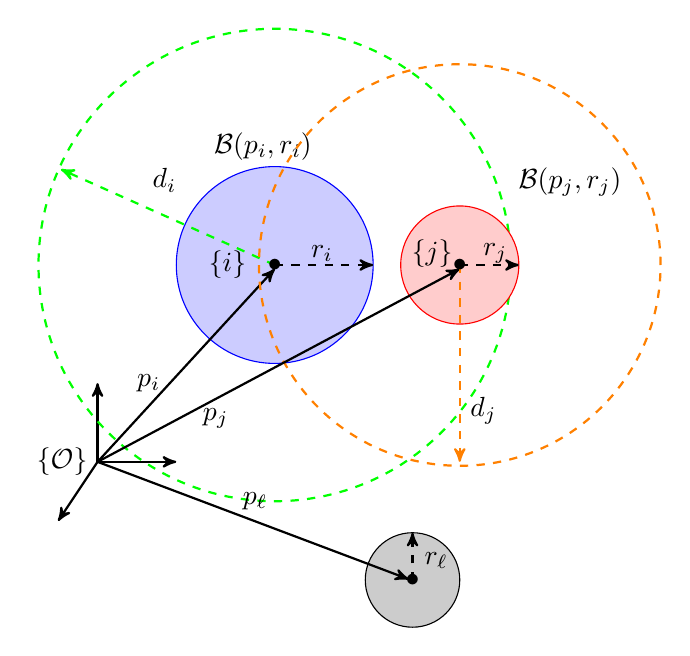
\begin{tikzpicture}[scale = 0.5]
	%draw the global frame
	\draw [color=black,thick,->,>=stealth'](-9, -5) to (-7, -5);
	\draw [color=black,thick,->,>=stealth'](-9, -5) to (-9, -3);
	\draw [color=black,thick,->,>=stealth'](-9, -5) to (-10, -6.5);
  \node at (-9.9, -5.0) {$\{\mathcal{O}\}$};

	%draw agent i
	\draw [color = blue, fill = blue!20] (-4.5,0) circle (2.5cm);
  \node at (-5.7, 0.0) {$\{i\}$};
	\draw[green,thick,dashed] (-4.5,0) circle (6.0cm);
	\draw [color=black,thick,->,>=stealth'](-9, -5) to (-4.5, -0.1);
	\node at (-7.7, -3.0) {$p_i$};
	\draw [color=green,thick,dashed,->,>=stealth'](-4.5, 0.0) to (-9.93, 2.43);
	\node at (-7.3, 2.15) {$d_i$};
	\draw [color=black,thick,dashed,->,>=stealth'](-4.5, 0.0) to (-2.0, 0.0);
	\node at (-3.3, 0.3) {$r_i$};
	\node at (-4.5, 0.0) {$\bullet$};
	\node at (-4.8, 3.0) {$\mathcal{B}(p_i, r_i)$};

	%draw agent j
	\draw [color = red, fill = red!20] (0.2, 0) circle (1.5cm);
	\node at (-0.5, 0.3) {$\{j\}$};
	\draw[orange,thick,dashed,] (0.2, 0) circle (5.1cm);
	\draw [color=black,thick,->,>=stealth'](-9, -5) to (0.2, -0.1);
	\node at (-6.0, -3.9) {$p_j$};
	\draw [color=orange,thick,dashed,->,>=stealth'](0.2, 0.0) to (0.2, -5.0);
	\node at (0.8, -3.7) {$d_j$};
	\draw [color=black,thick,dashed,->,>=stealth'](0.2, 0.0) to (1.7, 0.0);
	\node at (1.1, 0.3) {$r_j$};
	\node at (0.2, 0.0) {$\bullet$};
	\node at (3.0, 2.1) {$\mathcal{B}(p_j, r_j)$};

	% draw the obstacle
	\draw [color = black, fill = black!20] (-1, -8) circle (1.2cm);
	\draw [color=black,thick,->,>=stealth'](-9, -5) to (-1.1, -7.98);
	\draw [color=black,thick,dashed,->,>=stealth'](-1, -8) to (-1, -6.8);
	\node at (-1, -8) {$\bullet$};
	\node at (-5.0, -6.0) {$p_{\ell}$};
	\node at (-0.40, -7.5) {$r_{\ell}$};
\end{tikzpicture}

    \caption{Illustration of two agents $i, j \in \mathcal{V}$ and a static
      obstacle $\ell \in \mathcal{L}$ in the workspace; $\{\mathcal{O}\}$ is the inertial
      frame, $\{i\}, \{j\}$ are the frames attached to the agents' center of
      mass, $\vect{p}_i, \vect{p}_j, \vect{p}_{\ell} \in \mathbb{R}^3$ are the
      positions of the centers of mass of agents $i,j$ and obstacle $\ell$
      respectively, expressed in frame $\{\mathcal{O}\}$. $r_i, r_j, r_{\ell}$
      are the radii of the agents $i,j$ and the obstacle $\ell$ respectively.
      $d_i, d_j$ with $d_i > d_j$ are the agents' sensing ranges.
      In this figure, agents $i$ and $j$ are neighbours, since the center
      of mass of agent $j$ is within the sensing range of agent $i$ and vice
      versa: $\vect{p}_j \in \mathcal{B}\big(\vect{p}_i(t), d_i\big)$ and
      $\vect{p}_i \in \mathcal{B}\big(\vect{p}_j(t), d_j\big)$. Furthermore, the
      configuration between the two agents and the obstacle is a collision-free
      configuration.}
	\label{fig:two_agents_one_obstacle}
\end{figure}

Let us now define the distance between any two agents $i,j$ at time $t$ as
$d_{ij,a}(t)$; that between agent $i$ and obstacle $\ell$ as $d_{i\ell,o}(t)$;
and that between an agent $i$ and the origin of the workspace $W$ as
$d_{i,W}(t)$, with $d_{ij,a}, d_{i\ell,o}, d_{i,W} : \mathbb{R}^3 \to \mathbb{R}_{\geq 0}$:
\begin{subequations}
	\begin{align}
    d_{ij,a}(t) &\triangleq \| \vect{p}_i(t) - \vect{p}_j(t) \| \\[2.5ex]
    d_{i\ell,o}(t) &\triangleq \| \vect{p}_i(t) - \vect{p}_\ell(t) \| \\[2.5ex]
    d_{i,W}(t) &\triangleq \| \vect{p}_W - \vect{p}_i(t) \|
	\end{align}
\end{subequations}
as well as constants
\begin{subequations}
	\begin{align}
    \underline{d}_{ij, a} &\triangleq r_{i} + r_{j} \\[2.5ex]
    \underline{d}_{i\ell, o} &\triangleq r_{i} + r_{\ell} \\[2.5ex]
    \overline{d}_{i,W} &\triangleq r_W - r_i
	\end{align}
\end{subequations}
$\forall i, j \in \mathcal{V}$, $i \neq j$, $\ell \in \mathcal{L}$.
The latter stand for the minimum distance between two \textit{agents}, the
minimum distance between an \textit{agent} and an \textit{obstacle},
and the maximum distance between an \textit{agent} and the origin of the
workspace, respectively. They arise spatially as physical limitations and will
be utilized in forming collision-avoidance constraints.

Based on these definitions, we will now define the concept of a
\textit{collision-free configuration}:
\begin{bw_box}
\begin{definition} (\textit{Collision-free Configuration})
\label{definition:collision_free_conf}
  A collision-free configuration between
  \begin{itemize}
    \item any two agents $i,j \in \mathcal{V}$ is when $d_{ij,a}(t) > \underline{d}_{ij,a}$
    \item an agent $i \in \mathcal{V}$ and an obstacle $\ell \in \mathcal{L}$
     is when $d_{il,o}(t) > \underline{d}_{il,o}$
    \item an agent $i \in \mathcal{V}$ and the workspace $W$ boundary,
     is when $d_{i,W}(t) < \overline{d}_{i,W}$
  \end{itemize}
  at a generic time instant $t \in \mathbb{R}_{\geq 0}$. When all three
  conditions are met, we will simply refer to the overall configuration as
  a collision-free configuration.
\end{definition}
\end{bw_box}

    \subsection{Problem Statement}
Due to the fact that the agents are not dimensionless and their communication
capabilities are limited, the control protocol should for all neighboring
agents $i \in \mathcal{V}, j \in \mathcal{N}_i$ make sure that:

\begin{enumerate}
  \item the desired position formation $\vect{p}_{ij, \text{des}}$ is achieved
    in finite time
  \item the desired formation angles $\vect{q}_{ij, \text{des}}$ are achieved
    in finite time
  \item connectivity between initially connected agents (neighbours) is
    maintained at all times, i.e. all edges of $\mathcal{G}(t=0)$ are maintained
\end{enumerate}
Furthermore, for all agents $i \in \mathcal{V}$, obstacles $k \in \mathcal{K}$
and the workspace boundary $W$, it should guarantee for all
$t\in\mathbb{R}_{\geq 0}$ that:

\begin{enumerate}
  \item all agents avoid collision with each other
  \item all agents avoid collision with all obstacles
  \item all agents avoid collision with the workspace boundary
  \item singularity of the Jacobian matrices $\mat{J}_i$ is avoided
\end{enumerate}

Therefore, all neighboring agents of agent $i$ must remain within a distance
less than $d_i$ from him, for all $i \in \mathcal{V}$,
and all agents $i, j\in \mathcal{V}, i \neq j$ must remain within distance
greater than $\underline{d}_{ij,a}$ with one another.

Formally, the control problem under the aforementioned constraints is
formulated as follows:

\begin{bg_box}
\begin{problem}
  Consider $N$ agents modeled as bounded spheres $\mathcal{B}(\vect{p}_i, r_i)$,
  $i \in \mathcal{V}, |V| = N$ that operate in workspace $W$ that is also modeled
  as a bounded sphere $\mathcal{B}(0,r_W)$, featuring $|\mathcal{K}|$ spherical obstacles,
  also modeled as bounded spheres $\mathcal{B}(p_k, r_k), k \in \mathcal{K}$.
  Each agent $i$ is governed by the dynamics \eqref{eq:system}, under assumptions
  \ref{ass:measurements_access}, \ref{ass:initial_conditions},
  \ref{ass:after_formation_geometry}. Given desired \textit{feasible}
  inter-agent displacements $\vect{p}_{ij,des}$, $\vect{q}_{ij,des}$,
  $\forall i \in \mathcal{V}, j \in \mathcal{N}_i$ such that

  $$\underline{d}_{ij,a} < d_{ij,a} < d_i, \forall (i,j) \in
  \{(i,j) \in \mathcal{V} \times \mathcal{V}:
  \|\vect{p}_i - \vect{p}_j - \vect{p}_{ij,des}\| = 0\}$$

  design decentralized control laws $\vect{u}_i \in \mathbb{R}^6$ such that
  $\forall i \in \mathcal{V}$ and $t \in \mathbb{R}_{\geq 0}$ the following
  hold:

  \begin{enumerate}

    \item Position and orientation formation is achieved in steady-state
      $$\lim_{t \to \infty} \|\vect{x}_i(t) - \vect{x}_j(t) - \vect{x}_{ij,des}(t)\| < \mu_i,
        \forall j \in \mathcal{N}_i$$

    \item Inter-agent collision is avoided
      $$\|\vect{p}_i(t) - \vect{p}_j(t)\| > \underline{d}_{ij,a},
      \forall j \in \mathcal{V} \backslash \{i\}$$

    \item Agent-with-obstacle collision is avoided
      $$\|\vect{p}_i(t) - \vect{p}_k(t)\| > \underline{d}_{ik,o},
      \forall k \in \mathcal{K}$$

    \item Agent-with-workspace-boundary collision is avoided
      $$\|\vect{p}_i(t)\| + r_i < r_W$$

    \item Inter-agent connectivity loss is avoided
      $$\|\vect{p}_i(t) - \vect{p}_j(t)\| < d_i,
      \forall j \in \mathcal{N}_i$$

    \item All maps $\mat{J}_i$ are well defined
      $$\theta_i(t) \ne \pm \frac{\pi}{2}$$

  \end{enumerate}
\label{problem}
\end{problem}
\end{bg_box}

    \newpage

%-------------------------------------------------------------------------------
\part{Advocated Solutions}
\newpage

  \section{The model}
    \label{sec:the_model}

    We begin by rewriting the system equations \eqref{eq:system_1},
\eqref{eq:system_2} for a generic agent $i \in \mathcal{V}$ in state-space form:
\begin{subequations}
\begin{align}
  \dot{\vect{x}}_i(t) &= \mat{J}_i^{-1}(\vect{x}_i) \vect{v}_i(t) \\
  \dot{\vect{v}}_i(t) &= -\mat{M}_i^{-1}(\vect{x}_i)\mat{C}_i(\vect{x}_i,\dot{\vect{x}}_i) \vect{v}_i(t)
    - \mat{M}_i^{-1}(\vect{x}_i)\vect{g}_i(\vect{x}_i)
    + \mat{M}_i^{-1}(\vect{x}_i)\vect{u}_i
\end{align}
\label{eq:state_space_system}
\end{subequations}
where the inversion of $\mat{M}_i$ is possible due to it being
positive-definite $\forall i \in \mathcal{V}$. Denoting $\vect{z}_i(t)$ by
\begin{align}
  \vect{z}_i(t) =
    \begin{bmatrix}
      \vect{x}_i(t) \\
      \vect{v}_i(t) \\
    \end{bmatrix}
\end{align}
and
$\dot{\vect{x}}_i(t)$ and $\dot{\vect{v}}_i(t)$ by
\begin{subequations}
\begin{align}
  \dot{\vect{x}}_i(t) &= f_{i,x}(\vect{z}_i, \vect{u}_i) \\
  \dot{\vect{v}}_i(t) &= f_{i,v}(\vect{z}_i, \vect{u}_i)
\end{align}
\end{subequations}
we get the compact representation of the system's model
\begin{align}
  \dot{\vect{z}}_i(t) =
    \begin{bmatrix}
      f_{i,x}(\vect{z}_i, \vect{u}_i) \\
      f_{i,v}(\vect{z}_i, \vect{u}_i)
    \end{bmatrix} =
 f_i \big(\vect{z}_i (t), \vect{u}_i (t)\big)
\end{align}
The state evolution of agent $i$ is modeled by a system of non-linear
continuous-time differential equations of the form
\begin{align}
  \dot{\vect{z}}_i(t) &= f_i \big(\vect{z}_i (t), \vect{u}_i (t)\big) \label{eq:non_perturbed_system}\\
  \vect{z}_i(0) &= \vect{z}_{i,0} \\
  \vect{z}_i (t) & \in \mathcal{Z}_i \subset \mathbb{R}^{9} \times \mathbb{T}^3 \\
  \vect{u}_i (t) & \in \mathcal{U}_i \subset \mathbb{R}^6
\end{align}
where state $\vect{z}_i$ is directly measurable. It should be noted that
equation \eqref{eq:non_perturbed_system} does not consider model-plant
mismatches or external disturbances. The applied input $\vect{u}_i$ is a
portion of the optimal solution to an optimization problem where information on
the states of the neighbouring agents of agent $i$ are taken into account only
in the constraints considered in the optimization problem. These constraints
pertain to the set of its neighbours $\mathcal{N}_i$ and, in total, to the
set of all agents within its sensing range $\mathcal{R}_i$. Regarding these, we
make the following assumption:

\begin{gg_box}
\begin{assumption}
Considering the context of Model Predictive Control, when
at time $t_k$ agent $i$ solves a finite horizon optimization problem, it has
access to\footnote{Although
  $\mathcal{N}_i \subseteq \mathcal{R}_i$, we make the distinction between
  the two because all agents $j \in \mathcal{R}_i$ need to avoid collision
  with agent $i$, but only agents $j' \in \mathcal{N}_i$ need to remain
  within the sensing range of agent $i$. The distinction will prove the
  justification of its existence when considering the state constraints
  in the subsequent declaration of the optimization problem.}

\begin{enumerate}
  \item measurements of the states
    \begin{itemize}
      \item $\vect{z}_j(t_k)$ of all agents $j \in \mathcal{R}_i(t_k)$ within its sensing range at time $t_k$
      \item $\vect{z}_{j'}(t_k)$ of all of its neighbouring agents $j' \in \mathcal{N}_i$ at time $t_k$
      \end{itemize}
    \item the \textit{predicted states}
      \begin{itemize}
        \item $\overline{\vect{z}}_j(\tau)$ of all agents $j \in \mathcal{R}_i(t_k)$ within its sensing range
        \item $\overline{\vect{z}}_{j'}(\tau)$ of all of its neighbouring agents $j' \in \mathcal{N}_i$
      \end{itemize}
      across the entire horizon $\tau \in [t_k + h, t_k + T_p]$, where $T_p$ is the
      set time-horizon and $h$ is the sampling time.
\end{enumerate}
\end{assumption}
\end{gg_box}
We assume that these pieces of information are (a) always available and
accurate, and (b) exchanged without delay. We encapsulate these pieces of
information in four stacked vectors:
\begin{subequations}
\begin{align}
  \vect{z}_{\mathcal{R}_i}(t_k) &\triangleq col[\vect{z}_j(t_k)], \forall j \in \mathcal{R}_i(t_k) \\
  \vect{z}_{\mathcal{N}_i}(t_k) &\triangleq col[\vect{z}_j(t_k)], \forall j \in \mathcal{N}_i \\
  \overline{\vect{z}}_{\mathcal{R}_i}(\tau) &\triangleq col[\overline{\vect{z}}_j(\tau)], \forall j \in \mathcal{R}_i(t_k), \tau \in [t_k, t_k + T_p] \\
  \overline{\vect{z}}_{\mathcal{N}_i}(\tau) &\triangleq col[\overline{\vect{z}}_j(\tau)], \forall j \in \mathcal{N}_i, \tau \in [t_k, t_k + T_p]
\end{align}
\end{subequations}

The set $\mathcal{Z}_i$ captures all the state constraints of the system's
dynamics posed by the problem \eqref{problem}, not only for time $t_k$, but
over the entire prediction horizon $t \in [t_k, t_k + T_p]$.
Therefore $\mathcal{Z}_i$ is such that:
\begin{align}
  \mathcal{Z}_i = \{\overline{\vect{z}}_i \in \mathbb{R}^{9}\times \mathbb{T}^3 : \
      & \|\overline{\vect{p}}_i(t) - \overline{\vect{p}}_j(t)\| > \underline{d}_{ij,a}, \forall j \in \mathcal{R}_i(t), \label{constraint:p_1}\\
      & \|\overline{\vect{p}}_i(t) - \overline{\vect{p}}_j(t)\| < d_i, \forall j \in \mathcal{N}_i, \\
      & \|\overline{\vect{p}}_i(t) - \vect{p}_{\ell}\| > \underline{d}_{i\ell,o}, \forall \ell \in \mathcal{L}, \\
      & \|\vect{p}_W - \overline{\vect{p}}_i(t)\| < \overline{d}_{i,W}, \\
      & - \frac{\pi}{2} < \overline{\theta}_i(t) < \frac{\pi}{2} \label{constraint:p_5}, \\
  &\forall t \in [t_k, t_k + T_p]\}
\end{align}

Considering that $\mathcal{N}_i \subseteq \mathcal{R}_i$, that the state
vectors $\vect{z}_j$ are comprised of 12 real numbers that are encoded by
4 bytes, and that sampling occurs with a frequency $f$ for all agents, the
overall downstream bandwidth required by each agent is
$$BW_d = 12 \times 32\ \text{[bits]} \times |\mathcal{R}_i| \times \dfrac{T_p}{h} \times f\ [\text{sec}^{-1}]$$
Given conservative constants $f = 100$ Hz, $\dfrac{T_p}{h} = 100$, the
wireless protocol IEEE 802.11n-2009 (a standard for present-day devices)
can accomodate

$$|\mathcal{R}_i| = \dfrac{600\ [\text{Mbit}\cdot \text{sec}^{-1}] }{12\times32[\text{bit}]\times10^4 [\text{sec}^{-1}]} \sim
16 \cdot 10^2 \text{ agents}$$ within the range of one agent.
We deem this number to be large enough for practical applications
for the approach of assuming access to the predicted states of agents
within the range of one agent to be legal.

    \newpage

  \section{Position-based formation}
    \label{sec:position_based_solution}

    Here we are interested in steering each agent $i \in \mathcal{V}$ into
resting at a \textit{position} in 3D space, while conforming to the requirements
of the problem; that is, all agents should avoid colliding with each other, all
obstacles in the workspace, and the workspace boundary itself, while remaining
in a non-singular configuration and sustaining the connectivity to their
respective neighbours.


\subsection{The error model}

A desired configuration $\vect{z}_{i,des} \in \mathbb{R}^9 \times \mathbb{T}^3$
is associated to each agent $i \in \mathcal{V}$, with the aim of agent $i$
achieving it in steady-state:
$\lim\limits_{t \to \infty} \|\vect{z}_i(t) - \vect{z}_{i,des}\| = 0$. The
interior of this expression denotes the state error of agent $i$:

$$\vect{e}_i(t) = \vect{z}_i(t) - \vect{z}_{i,des}, \vect{e}_i(t) :
\mathbb{R}_{\geq 0} \to \mathbb{R}^9 \times \mathbb{T}^3$$

The error dynamics are denoted by $g_i(\vect{e}_i, \vect{u}_i)$:
\begin{align}
  \dot{\vect{e}}_i(t) = \dot{\vect{z}}_i(t) - \dot{\vect{z}}_{i,des} =
  \dot{\vect{z}}_i(t) = f_i(\vect{z}_i(t), \vect{u}_i(t)) = g_i(\vect{e}_i(t), \vect{u}_i(t))
  \label{eq:position_based_error_model}
\end{align}
with $\vect{e}_i(0) = \vect{z}_i(0) - \vect{z}_{i,des}$


\subsection{The optimization problem}

At a generic time $t_0$, agent $i$ solves the following optimization problem:

\begin{align}
  \min\limits_{\overline{\vect{u}}_i (\cdot)}\ &
    J_i \big(\overline{\vect{u}}_i (\cdot);\ \vect{e}_i(t_0)) \triangleq
      \int_{t_0}^{t_0 + T_p} F_i \big(\overline{\vect{e}}_i(\tau), \overline{\vect{u}}_i (\tau)\big) d \tau +
      V_i \big(\overline{\vect{e}}_i (t_0 + T_p)\big) \label{position_based_cost} \\
  \text{subject to:} & \nonumber \\
  & \dot{\overline{\vect{e}}}_i(t) = g_i (\overline{\vect{e}}_i (t), \overline{\vect{u}}_i (t)) \\
  & \overline{\vect{e}}_i (t_0) = \vect{e}_i (t_0) \\
  & \overline{\vect{u}}_i(t) \in \mathcal{U}_i, t \in [t_0, t_0 + T_p)\\
  & \overline{\vect{e}}_i (t) \in \mathcal{E}_i,\ t \in [t_0, t_0 + T_p]\\
  & \overline{\vect{e}}_i (t_0 + T_p) \in \mathcal{E}_i^f \\
  \text{and } \forall t \in [t_0, t_0 + T_p]:& \nonumber \\
  & \|\overline{\vect{p}}_i(t) - \overline{\vect{p}}_j(t)\| > \underline{d}_{ij,a}, \forall j \in \mathcal{R}_i(t) \label{constraint:p_1}\\
  & \|\overline{\vect{p}}_i(t) - \vect{p}_k(t)\| > \underline{d}_{ik,o}, \forall k \in \mathcal{K} \\
  & \|\overline{\vect{p}}_i(t)\| + r_i < r_W \\
  & \|\overline{\vect{p}}_i(t) - \overline{\vect{p}}_j(t)\| < d_i, \forall j \in \mathcal{N}_i \\
  & \overline{\theta}_i(t) \ne \pm \frac{\pi}{2} \label{constraint:p_5}
\end{align}\\
Constraints \ref{constraint:p_1}-\ref{constraint:p_5} explicitly address the
requirements posed by the problem \eqref{problem}, while the rest exist to
ensure that formation is achieved under constrained states and input signals.

The functions
$F_i : \mathcal{E}_i \times \mathcal{U}_i \to \mathbb{R}_{\geq 0}$ and
$V_i: \mathcal{E}_i^f \to \mathbb{R}_{\geq 0}$ are defined as
\begin{align}
  F_i (\vect{e}_i, \vect{u}_i)
    &\triangleq \| \vect{e}_i\|_{\mat{Q}_i}^2 + \| \vect{u}_i\|_{\mat{R}_i}^2 \\
  V_i (\vect{e}_i)
    & \triangleq \| \vect{e}_i \|_{\mat{P}_i}^2
\end{align}\\
Matrices $\mat{R}_i \in \mathbb{R}^{6 \times 6}$ are symmetric and positive
definite, while matrices $\mat{Q}_i, \mat{P}_i \in \mathbb{R}^{12 \times 12}$
are symmetric and positive semi-definite.

The set $\mathcal{E}_i$ is such that
$$\mathcal{E}_i = \{\vect{e}_i \in \mathbb{R}^{12} : \vect{e}_i \in \mathcal{Z}_i \oplus (-z_{i,des} )\}$$

The set $\mathcal{E}_i^f \subseteq \mathcal{E}_i$ is an admissible positively
invariant set \note{?? define it} for system \eqref{eq:position_based_error_model}
such that
\begin{align}
  \mathcal{E}_i^f = \{\vect{e}_i \in \mathcal{E}_i : \|\vect{e}_i\| \leq \epsilon_0 \}
\end{align}
where $\epsilon_0$ is an arbitrarily small but fixed positive real scalar.\\

The solution to the optimal control problem \eqref{position_based_cost} -
\eqref{constraint:p_5} at time $t_0$ is an optimal control input
$\vect{u}_i^{\ast}(t;\ \vect{e}_i(t_0))$, with $t \in [t_0, t_0 + T_p]$, which
is applied to the open-loop system until the next sampling instant $t_0 + h$:
\begin{align}
  \vect{u}_i(t;\ \vect{e}_i(t_0)) = \vect{u}_i^{\ast}(t_0;\ \vect{e}_i(t_0)) \\
  t \in [t_0, t_0 + h) \\
  0 < h < T_p
\end{align}

The control input $\vect{u}_i(\cdot)$ is a feedback, since it is
recalculated at each sampling instant based on the then-current state. The
solution to equation \eqref{eq:position_based_error_model}, starting at time
$t_0$, from an initial condition $\vect{e}_i(t_0)$, by application of the
control input $\vect{u}_i : [t_0, t_1] \to \mathcal{U}_i$ is denoted by
$$\vect{e}_i(\tau;\ \vect{u}_i(\cdot), \vect{e}_i(t_0))$$
with $\tau \in [t_0, t_1]$.

The \textit{predicted} state of the system \eqref{eq:position_based_error_model}
at time $t_0 + \tau$, based on the measurement of the state at time
$t_0$, $\vect{e}_i(t_0)$, by application of the control input
$\vect{u}_i(t;\ \vect{e}_i(t_0))$, for the time period $t \in [t_0, t_0 + \tau]$
is denoted by
$$\overline{\vect{e}}_i(t_0 + \tau;\ \vect{u}_i(\cdot), \vect{e}_i(t_0))$$
As is natural,
$\vect{e}_i(t_0) = \overline{\vect{e}}_i(t_0;\ \vect{u}_i(\cdot), \vect{e}_i(t_0))$.\\

We can now give the definition of an \textit{admissible input}:

\begin{bw_box}
\begin{definition} (Admissible input)\\

  A control input $\vect{u}_i : [0, T_p] \to \mathbb{R}^6$ for a state
  $\vect{e}_i(t_0)$ is called \textit{admissible} if all the following hold:

  \begin{enumerate}
    \item $\vect{u}_i(\cdot)$ is piecewise continuous
    \item $\vect{u}_i(\tau) \in \mathcal{U},\ \forall \tau \in [t_0, t_0 + T_p]$
    \item $\vect{e}_i(\tau;\ \vect{u}_i(\cdot), \vect{e}_i(t_0)) \in \mathcal{E}_i,\ \forall \tau \in [t_0, t_0 + T_p]$
    \item $\vect{e}_i(T_p;\ \vect{u}_i(\cdot), \vect{e}_i(t_0)) \in \mathcal{E}_i^f$
  \end{enumerate}

\end{definition}
\end{bw_box}


\begin{bw_box}
\begin{theorem} Suppose that

  \begin{enumerate}
    \item The optimal control problem \eqref{position_based_cost} -
      \eqref{constraint:p_5} is feasible at time $t=0$, that is, assumptions
      \eqref{ass:measurements_access}, \eqref{ass:initial_conditions}, and
      \eqref{ass:after_formation_geometry} hold at time $t=0$
    \item
  \end{enumerate}

\end{theorem}
\end{bw_box}



\begin{gg_box}
\begin{assumption} (Functions $g_i$ are Lipschitz continuous)
  \label{ass:g_i_Lipschitz}
\end{assumption}
\end{gg_box}

\begin{gg_box}
\begin{assumption} (Functions $F_i$ are Lipschitz continuous)
  \label{ass:F_i_Lipschitz}
\end{assumption}
\end{gg_box}


\begin{gg_box}
\begin{assumption} (Functions $V_i$ are Lipschitz continuous)
  \label{ass:V_i_Lipschitz}
\end{assumption}
\end{gg_box}

    \newpage

  \section{Displacement-based formation}
    \label{sec:displacement_based_solution}

    \subsection{Cost function}

\begin{align}
  J_i \big(\overline{\vect{u}}_i (\cdot);\ \vect{z}_i(t_0), \vect{z}_{\mathcal{N}_i}(t_0)\big) &\triangleq
    J_i^U \big(\overline{\vect{u}}_i (\cdot) \big) +
    J_i^Z \big(\vect{z}_i (t_0), \vect{z}_{\mathcal{N}_i}(t_0)\big)
\end{align}

where
\begin{align}
  J_i^U \big(\overline{\vect{u}}_i (\cdot)\big) &\triangleq
    \int_{t_0}^{t_0 + T_p} h_i \big(\overline{\vect{u}}_i (\tau)\big) d \tau \\
  J_i^Z \big(\vect{z}_i (t_0), \vect{z}_{\mathcal{N}_i}(t_0)\big) & \triangleq
    \sum_{j \in \mathcal{N}_i} \Bigg(\int_{t_0}^{t_0 + T_p} g_{ij} \big(\overline{\vect{z}}_i (\tau), \overline{\vect{z}}_j (\tau)\big) d \tau +
    V_{ij} \big(\overline{\vect{z}}_i (t_0 + T_p), \overline{\vect{z}}_j (t_0 + T_p)\big)\Bigg)
\end{align}
\note{without the sum maybe? (just in col form)}
and

\begin{align}
  h_i \big(\vect{u}_i(t) \big)
    &\triangleq \| \vect{u}_i(t)\|_{\mat{R}_i}^2 \\
  g_{ij}\big(\vect{z}_i(t), \vect{z}_j(t)\big)
    & \triangleq \| \vect{z}_i(t) - \vect{z}_j(t) - \vect{z}_{ji,des} \|_{\mat{G}_{ij}}^2 \\
  V_{ij} \big(\vect{z}_i (t_0 + T_p), \vect{z}_j (t_0 + T_p)\big)
    & \triangleq \| \vect{z}_i(t_0 + T_p) - \vect{z}_j(t_0 + T_p) - \vect{z}_{ji,des} \|_{\mat{P}_{ij}}^2
\end{align}\\
Matrices $\mat{R}_i \in \mathbb{R}^{6 \times 6}$ are symmetric and positive
definite, while matrices $\mat{G}_{ij}, \mat{P}_{ij} \in \mathbb{R}^{12 \times 12}$ are
symmetric and positive semi-definite.



\subsection{Optimization problem}

At a generic time $t_0$, agent $i$ solves the following optimization problem:

\begin{align}
  \min\limits_{\overline{\vect{u}}_i (\cdot)}\ &
    J_i \big(\overline{\vect{u}}_i (\cdot);\ \vect{z}_i(t_0), \vect{z}_{\mathcal{N}_i}(t_0)\big) \\
  \text{subject to:} & \\
  & \dot{\overline{\vect{z}}}_i(t) = f_i (\overline{\vect{z}}_i (t), \overline{\vect{u}}_i (t)) \\
  & \overline{\vect{z}}_i (t_0) = \vect{z}_i (t_0) \\
  & \overline{\vect{z}}_j (t_0) = \vect{z}_j (t_0), j \in \mathcal{N}_i \\
  & \overline{\vect{u}}_i(t) \in \mathcal{U}_i,\ j \in \mathcal{N}_i, t \in [t_0, t_0 + T_p)\\
  & \overline{\vect{z}}_i (t) - \overline{\vect{z}}_j (t) - z_{ji, des} \in \mathcal{Z}_i,\ t \in [t_0, t_0 + T_p]\\
  & \overline{\vect{z}}_i (t_0 + T_p) - \overline{\vect{z}}_j (t_0 + T_p) - z_{ji,des} \in \mathcal{Z}_i^f, j \in \mathcal{N}_i \\
  & \|\vect{p}_i(t) - \vect{p}_j(t)\| > \underline{d}_{ij,a}, \forall j \in \mathcal{R}_i(t), t \in [t_0, t_0 + T_p] \\
  & \|\vect{p}_i(t) - \vect{p}_k(t)\| > \underline{d}_{ik,o}, \forall k \in \mathcal{K}, t \in [t_0, t_0 + T_p] \\
  & \|\vect{p}_i(t)\| + r_i < r_W, t \in [t_0, t_0 + T_p] \\
  & \|\vect{p}_i(t) - \vect{p}_j(t)\| < d_i, \forall j \in \mathcal{N}_i, t \in [t_0, t_0 + T_p] \\
  & \theta_i(t) \ne \pm \frac{\pi}{2}, t \in [t_0, t_0 + T_p]
\end{align}

Constraints \ref{}-\ref{} explicitly address the
requirements posed by the problem \eqref{problem}, while the rest exist to
ensure that formation is achieved under constrained input signals.


\begin{gg_box}
\begin{assumption} (Functions $f_i$ are Lipschitz continuous)
  \label{ass:f_i_Lipschitz}
\end{assumption}
\end{gg_box}

\begin{gg_box}
\begin{assumption} (Functions $h_i$ are Lipschitz continuous)
  \label{ass:h_i_Lipschitz}
\end{assumption}
\end{gg_box}

\begin{gg_box}
\begin{assumption} (Functions $g_{ij}$ are Lipschitz continuous)
  \label{ass:g_ij_Lipschitz}
\end{assumption}
\end{gg_box}

\begin{gg_box}
\begin{assumption}

  There exists a local stabilizing controller
  $\vect{\kappa}_i(\vect{x}) \in \mathcal{U}_i$ such that

  \begin{align}
    \dfrac{\partial V_i}{\partial \vect{x}} f_i \Big(\vect{x}(\tau), \vect{\kappa}_i\big(\vect{x}(\tau)\big)\Big) +
      h_i\Big(\vect{x}(\tau), \vect{\kappa}_i \big(\vect{x}(\tau)\big)\Big) \leq 0, \forall \vect{x} \in \Phi_i
  \end{align}

  where $\Phi_i = \{\vect{x} \in \mathbb{R}^n : V_i(\vect{x}) \leq \alpha_i \}$, and
  $\Phi_i \subseteq \mathcal{X}_i^{T_p} = \{x \in \mathbb{R}^n : \vect{\kappa}_i(\vect{x}) \in \mathcal{U}_i\}$

  \label{ass:local_controller_k}
\end{assumption}
\end{gg_box}


\begin{gg_box}
\begin{assumption}

  The terminal costs $V_i(\vect{x})$ are Lipschitz continuous in $\vect{x} \in \Phi_i$
  with Lipschitz constants $L_{V_i}$:

  \begin{align}
    \| V_i(\vect{x}_1) - V_i(\vect{x}_2)\| \leq L_{V_i} \|\vect{x}_1 - \vect{x}_2 \|
  \end{align}

  \label{ass:V_i_Lipschitz}
\end{assumption}
\end{gg_box}


\begin{gg_box}
\begin{assumption}

  The terminal set $\mathcal{X}_{f_i} = \{ \vect{x} \in \mathbb{R}^n : V_i(\vect{x}) \in \alpha_{V_i}\}$
  is such that for all $\vect{x} \in \Phi_i$, $f_i\big(\vect{x}, \vect{\kappa}_i(\vect{x})\big) \in \mathcal{X}_{f_i} \subseteq \Phi_i$.

  \label{ass:x_f_i}
\end{assumption}
\end{gg_box}

    \newpage


\bibliography{references}
\bibliographystyle{ieeetr}

\end{document}
